\usetikzlibrary{positioning, arrows.meta, shapes.geometric}

\begin{figure}[h]
\centering
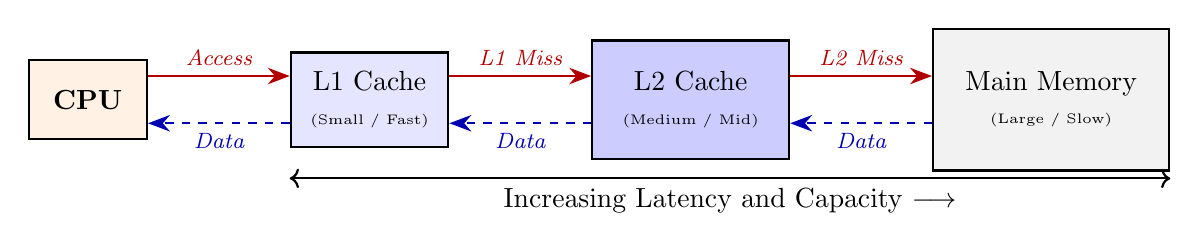
\begin{tikzpicture}[
    node distance=1.2cm and 1.8cm,
    cpu/.style={rectangle, draw, thick, fill=orange!10, minimum width=1.5cm, minimum height=1cm, font=\bfseries},
    l1/.style={rectangle, draw, thick, fill=blue!10, minimum width=2.0cm, minimum height=1.2cm, align=center},
    l2/.style={rectangle, draw, thick, fill=blue!20, minimum width=2.5cm, minimum height=1.5cm, align=center},
    mem/.style={rectangle, draw, thick, fill=gray!10, minimum width=3.0cm, minimum height=1.8cm, align=center},
    arrow_fwd/.style={-{Stealth[scale=1.2]}, thick, color=red!70!black},
    arrow_back/.style={-{Stealth[scale=1.2]}, thick, dashed, color=blue!70!black},
    label_style/.style={font=\footnotesize\itshape}
]

\node[cpu] (cpu) {CPU};
\node[l1, right=of cpu] (l1) {L1 Cache \\ \tiny (Small / Fast)};
\node[l2, right=of l1] (l2) {L2 Cache \\ \tiny (Medium / Mid)};
\node[mem, right=of l2] (mem) {Main Memory \\ \tiny (Large / Slow)};

\draw[arrow_fwd] ([yshift=3mm]cpu.east) -- ([yshift=3mm]l1.west) 
    node[midway, above, label_style] {Access};
\draw[arrow_fwd] ([yshift=3mm]l1.east) -- ([yshift=3mm]l2.west) 
    node[midway, above, label_style] {L1 Miss};
\draw[arrow_fwd] ([yshift=3mm]l2.east) -- ([yshift=3mm]mem.west) 
    node[midway, above, label_style] {L2 Miss};

\draw[arrow_back] ([yshift=-3mm]mem.west) -- ([yshift=-3mm]l2.east) 
    node[midway, below, label_style] {Data};
\draw[arrow_back] ([yshift=-3mm]l2.west) -- ([yshift=-3mm]l1.east) 
    node[midway, below, label_style] {Data};
\draw[arrow_back] ([yshift=-3mm]l1.west) -- ([yshift=-3mm]cpu.east) 
    node[midway, below, label_style] {Data};

\draw[thick, <->] ([yshift=-1cm]l1.west) -- ([yshift=-1cm]mem.east) 
    node[midway, below] {Increasing Latency and Capacity $\longrightarrow$};

\end{tikzpicture}
\end{figure}